\documentclass[10pt]{mypackage}

\usepackage[uprightgreeks,light]{kpfonts}
\renewcommand{\coloneq}{\coloneqq}
\usepackage{homework}
%\usepackage{notes}

%\usepackage[ backend=bibtex, style = alphabetic, sorting=ynt ]{biblatex}
%\addbibresource{  }

\usepackage{parskip}

\fancyhf{}
\fancyhead[R]{Avinash Iyer}
\fancyhead[L]{Algebraic Topology: Homework 23}
\fancyfoot[C]{\thepage}

\setcounter{secnumdepth}{0}

\begin{document}
\RaggedRight
\section{Revised Problems}%
\begin{problem}[Homework 17, Problem 1]
  Give two examples of a nontrivial covering space of the Klein bottle, one normal and one non-normal.
\end{problem}
\begin{solution}
As exhibited below, we can view the torus as a two-sheeted cover of the Klein bottle. Since the number of sheets is equal to the index of $p_{\ast}\left( \pi_1\left( \widetilde{X},\widetilde{x}_0 \right) \right)$ in $\pi_1\left( X,x_0 \right)$, and the covering map is injective, it follows that this is a normal covering since index $2$ subgroups are normal.
\begin{center}
  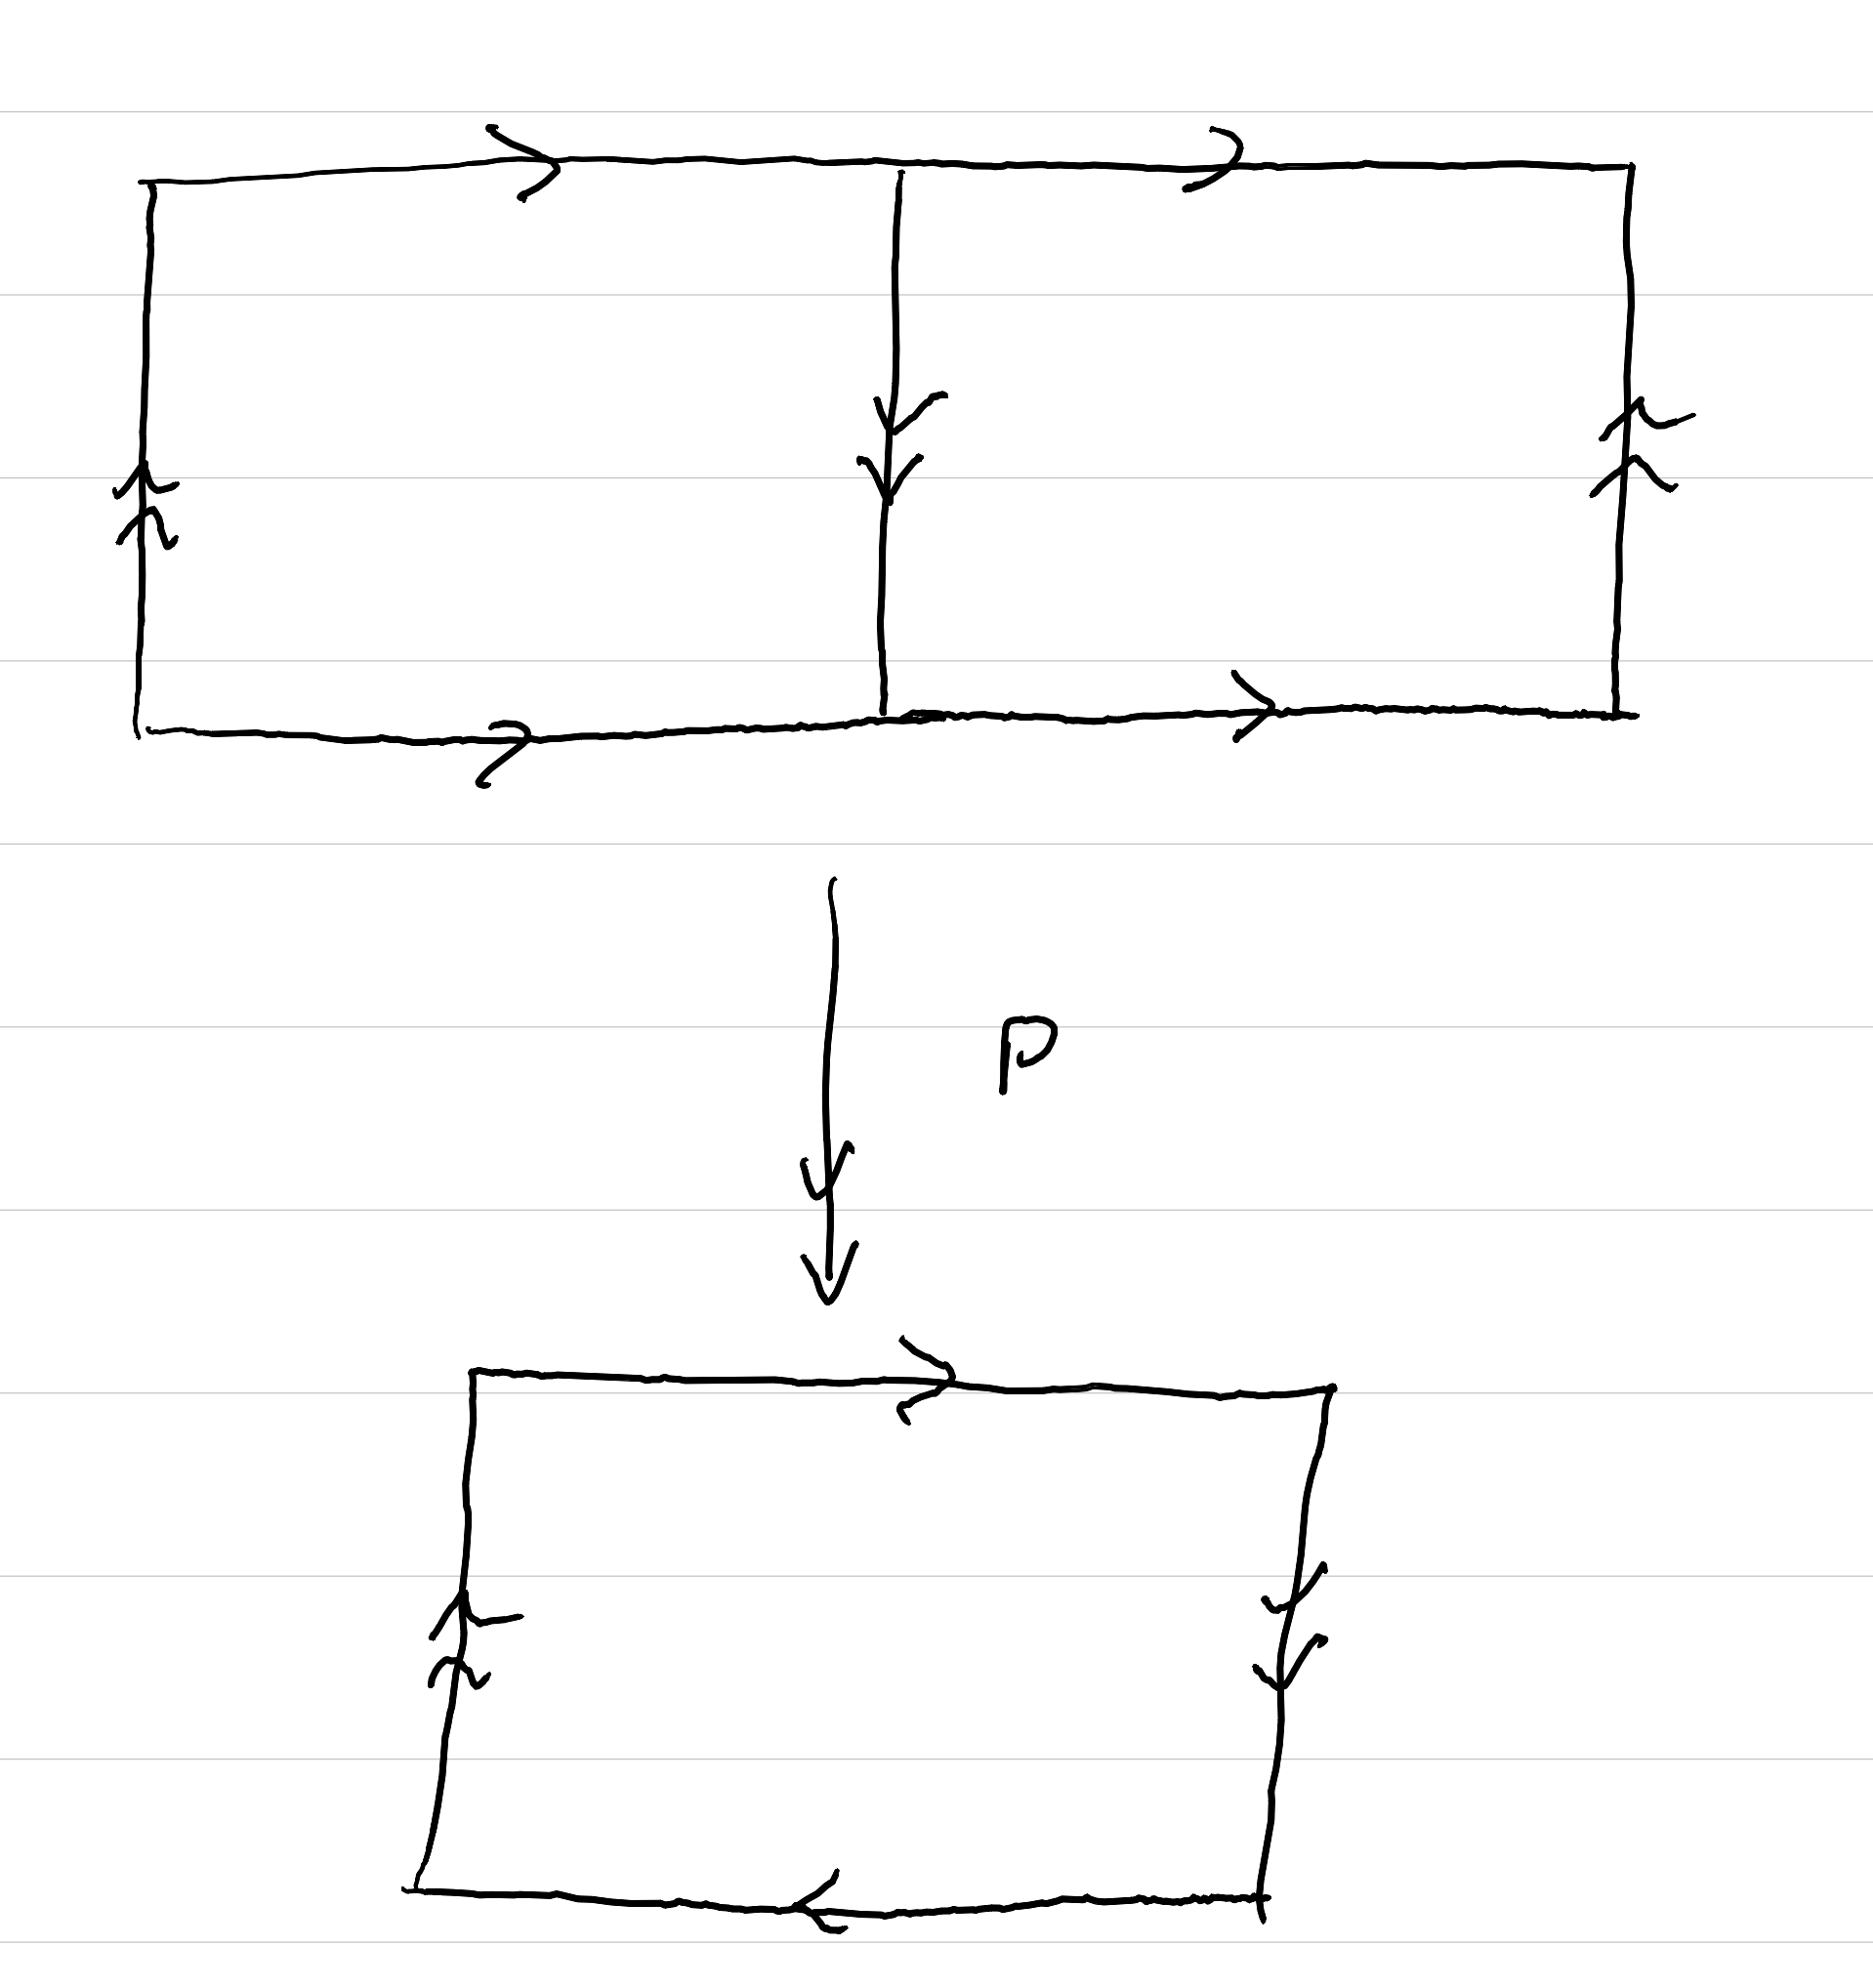
\includegraphics[width=7cm]{images/two_sheeted_klein_bottle.png}
\end{center}
Similarly, to find a non-normal covering, we consider the following three-sheeted covering space. This covering lifts the loop given by $a$ to three copies of itself, while it lifts $b$ to one copy of itself. In particular, this means that this cover corresponds to the subgroup of the Klein bottle group $\left\langle a,b|abab^{-1} \right\rangle$ given by $H = \left\langle a^3,b \right\rangle$. Yet, since $b\in H$, but $aba^{-1} = a\left( aba \right)a^{-1}=a^2b$, it follows that $H$ is not normal, so this is a non-normal covering space of the Klein bottle.
\begin{center}
  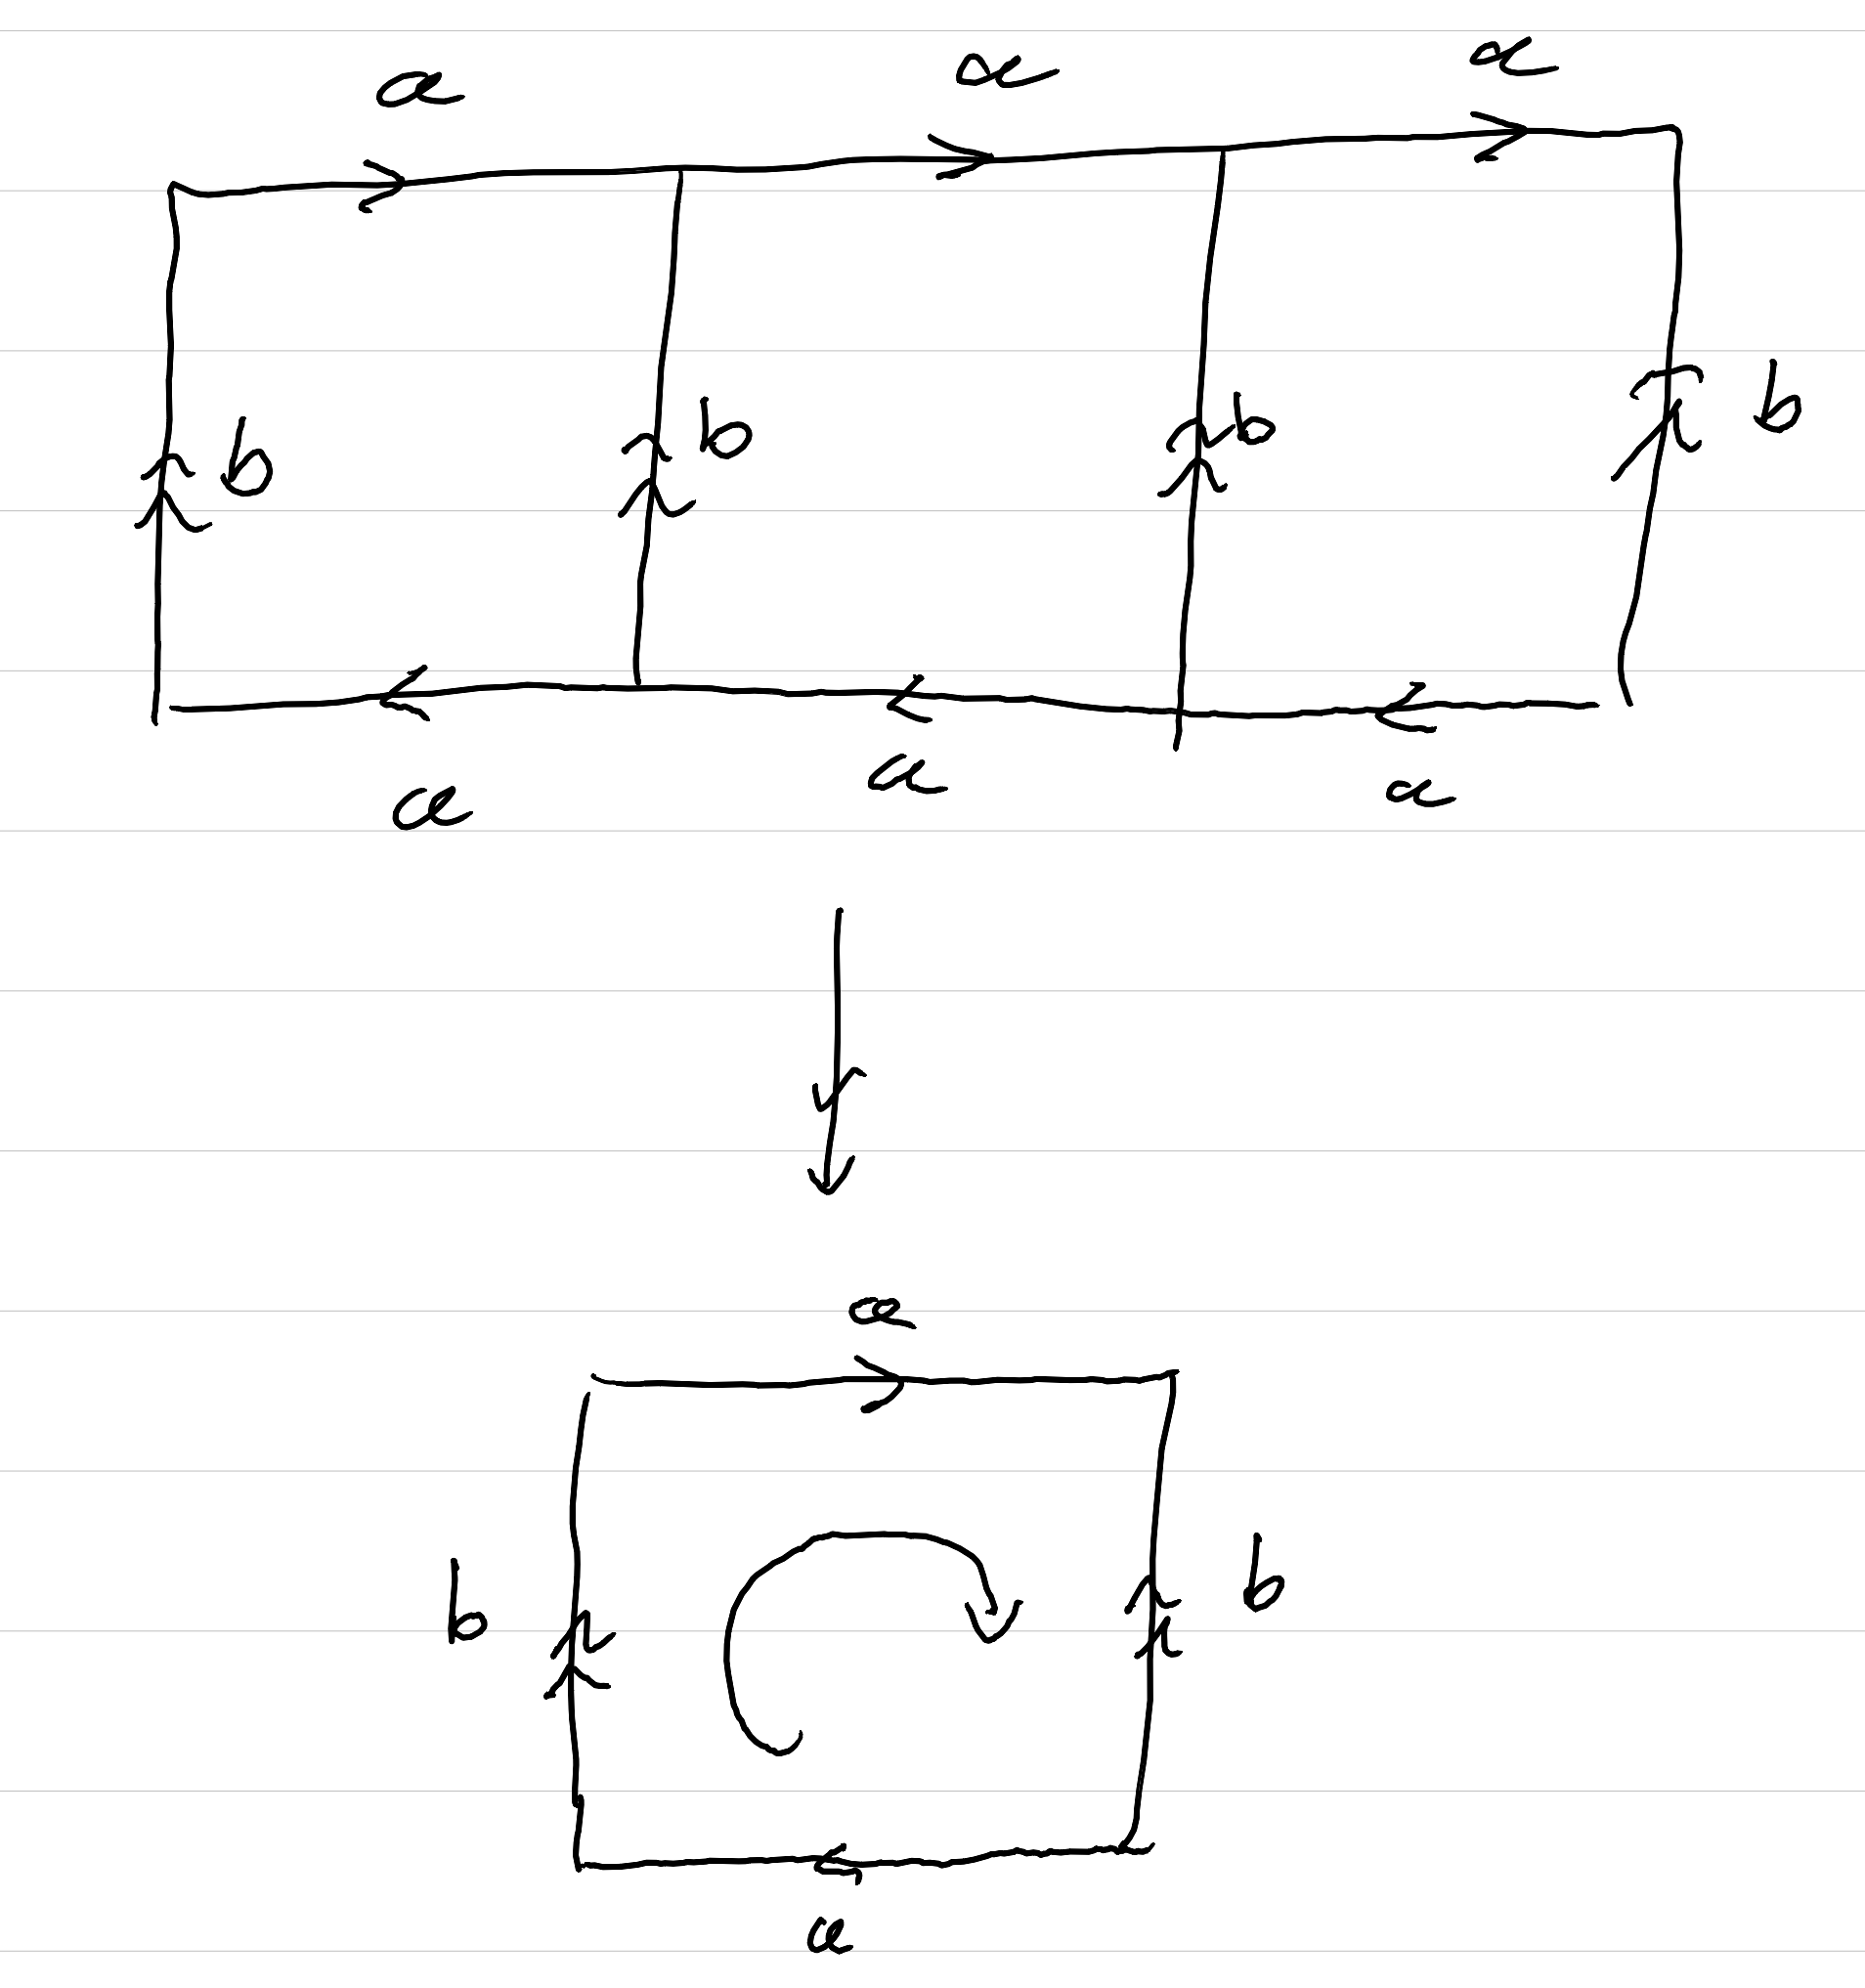
\includegraphics[width=7cm]{images/three_sheeted_klein_bottle.png}
\end{center}
\end{solution}
\section{Current Problems}%
\begin{problem}[Problem 1]
  Let $\left[ v_0,\dots,v_q \right]$ be a $q$-simplex in $\R^m$ for $m\geq q$. Prove that if $d$ is the diameter of a simplex in the barycentric subdivision of $\left[ v_0,\dots,v_q \right]$, then $d\leq \frac{q}{q+1} \operatorname{diam}\left( \left[ v_0,\dots,v_q \right] \right)$.
\end{problem}
\begin{solution}
  We claim that
  \begin{align*}
    \operatorname{diam}\left( \left[ v_0,\dots,v_q \right] \right) &= \max\set{\left\vert v_i-v_j \right\vert : 1\leq i<j\leq q}.
  \end{align*}
  This follows from the fact that if $u$ and $w$ are any two elements of $\Delta^q$, and $w$ has convex combination expression
  \begin{align*}
    w &= \sum_{i=0}^{q}s_iv_i,
  \end{align*}
  then
  \begin{align*}
    \left\vert u-w \right\vert &= \left\vert u-\sum_{i=0}^{q}s_iv_i \right\vert\\
                               &= \left\vert \sum_{i=0}^{q}s_i \left( u-v_i \right) \right\vert\\
                               &\leq \sum_{i=0}^{q} s_i \left\vert u-v_i \right\vert\\
                               &\leq \sum_{i=0}^{q} s_i \max_{i=0}^{q} \left\vert u-v_i \right\vert\\
                               &= \max_{i=0}^{q} \left\vert u-v_i \right\vert.
  \end{align*}
  In particular, this means that if $u\in \Delta^q$, then $\left\vert u-v_i \right\vert\leq \max\set{\left\vert v_i-v_j \right\vert : 1\leq i<j\leq q}$. Thus, this is in fact our desired diameter.

  Observe then that, if we set
  \begin{align*}
    b &= \frac{1}{q+1} \sum_{i=0}^{q}v_i,
  \end{align*}
  then for any $v_j$, we have
  \begin{align*}
    \left\vert b-v_j \right\vert &= \left\vert \frac{1}{q+1}\sum_{i=0}^{q}v_i - v_j \right\vert\\
                                 &= \left\vert \frac{1}{q+1} \sum_{i=0}^{q} \left( v_i-v_j \right) \right\vert\\
                                 &\leq \frac{1}{q+1} \sum_{i=0}^{q} \left\vert v_i-v_j \right\vert\\
                                 &= \frac{1}{q+1} \sum_{i\neq j} \left\vert v_i-v_j \right\vert\\
                                 &\leq \frac{1}{q+1} \sum_{i\neq j} \max\set{\left\vert v_i-v_j \right\vert : 1\leq i < j \leq q}\\
                                 &= \frac{q}{q+1} \operatorname{diam}\left( \left[ v_0,\dots,v_q \right] \right).
  \end{align*}
\end{solution}
\end{document}
